% VGG-T-Det fine-tuning data: is the ARKitScenes ground-truth box frame the same as ScanNet's? Findings and fixes.
% Fragment for % VGG-T-Det fine-tuning data: is the ARKitScenes ground-truth box frame the same as ScanNet's? Findings and fixes.
% Fragment for % VGG-T-Det fine-tuning data: is the ARKitScenes ground-truth box frame the same as ScanNet's? Findings and fixes.
% Fragment for % VGG-T-Det fine-tuning data: is the ARKitScenes ground-truth box frame the same as ScanNet's? Findings and fixes.
% Fragment for \input{vggt-det-training-data}; needs \usepackage{booktabs} and \usepackage{graphicx}.
% Figure file: vggt-det-training-data-overlay.jpg (same folder).
% Data: vggtdet_es56/data/scannet/scannet_infos_train_vsi63.pkl (958 scenes),
%       vggtdet_es56/data/arkit_r190k/arkit_infos_{train,val}_vsi63.pkl (2,267 / 562 scenes).
% Sources: vggtdet_es56/code/tools/vsi63/check_frames_{static,pipeline,model,overlay}.py, scannet_frame.py;
%          results in vggtdet_es56/runs/frame_check/{static,static_after,pipeline,pipeline_after,model}.json.
% Static checks: 150 random scenes per dataset. Pipeline check: 60 random training samples per dataset.

\section{Training data for VGG-T-Det: one box frame for ScanNet and ARKitScenes}
\label{sec:vggtdet-data}

\paragraph{Question.}
VGG-T-Det is fine-tuned on EmbodiedScan boxes of ScanNet (958 scenes) and ARKitScenes (2,267 scenes). The
ScanNet files come from the original VGG-T-Det release, the ARKitScenes files from our own converter. The two
must describe boxes in the same way, or the detector is trained on contradictory targets. We checked this with
several independent tests, each run identically on both datasets so that ScanNet's numbers are the reference.

\paragraph{What the detector's targets depend on.}
The head predicts a box centre in the frame of the first input image and maps it to the scene's aligned frame
with (alignment matrix) $\times$ (pose of the first image). Sizes are predicted directly along the aligned
frame's axes. The targets therefore depend on the rotation of the aligned frame (which way is up, whether the
walls lie on $x$ and $y$), the camera convention of the poses, the metric scale, and the box definition
(gravity centre, axis-aligned size). They do not depend on where the aligned frame's origin is: moving the
origin moves the alignment matrix and the boxes together, and the centre in the first image's frame stays the
same. The stored camera intrinsics are not used by the detector, which takes them from VGGT.

\paragraph{Result.}
The ARKitScenes boxes already agreed with ScanNet in everything the targets depend on. Two things differed,
and neither changed the targets:
\begin{itemize}
\item \textbf{Origin.} ScanNet's aligned frame has the floor at $z=0$ and the mean $x$, $y$ of the scene at 0.
The ARKitScenes files put the origin at the first camera of the trajectory, so the floor was at about
$-1.2$\,m.
\item \textbf{Focal length of portrait videos.} The converter scaled the sensor focal length by image width
over sensor width, which is correct for landscape videos and 0.75 times too small for portrait ones
(398 instead of 531 pixels for a $480\times640$ image). This affected 1,031 of the 2,267 training scenes.
\end{itemize}
Both are now corrected in the ARKitScenes training and validation files (Section~\ref{sec:vggtdet-data-fix}).
Checkpoints trained before the correction remain valid, because the targets are unchanged.

\subsection{Size of the training data}
\label{sec:vggtdet-data-size}

Table~\ref{tab:vggtdet-size} counts the scenes and boxes of the 65-class detector. ScanNet and ARKitScenes use
the EmbodiedScan boxes, ScanNet++ its own annotations. The ARKitScenes and ScanNet++ files include the scenes
built from the raw downloads (\texttt{*\_vsi65\_full.pkl}); before those were added there were 4,272 scenes and
79,670 boxes (ARKitScenes 2,267 / 562 scenes and 39,414 / 9,663 boxes, ScanNet++ 218 / 24 scenes and 7,139 / 742
boxes). Eleven more ARKitScenes training scenes were built but left out (ten with fewer than 42 frames, one without
a box of the 65 classes), and 605 downloaded ScanNet++ scenes lack camera poses. During training ARKitScenes is
validated on a subset of 187 scenes with 3,306 boxes.

\begin{table}[t]
\centering
\caption{Scenes and boxes of the 65-class VGG-T-Det training data (train / validation).}
\label{tab:vggtdet-size}
\begin{tabular}{lrrrrrr}
\toprule
 & \multicolumn{3}{c}{Scenes} & \multicolumn{3}{c}{Boxes} \\
\cmidrule(lr){2-4}\cmidrule(lr){5-7}
Dataset & Train & Val & Total & Train & Val & Total \\
\midrule
ScanNet (EmbodiedScan)     &   958 &   243 & 1,201 & 18,214 &  4,498 &  22,712 \\
ARKitScenes (EmbodiedScan) & 3,587 &   899 & 4,486 & 59,780 & 14,866 &  74,646 \\
ScanNet++                  &   227 &    24 &   251 &  7,543 &    742 &   8,285 \\
\midrule
Total                      & 4,701 & 1,237 & 5,938 & 85,537 & 20,106 & 105,643 \\
\bottomrule
\end{tabular}
\end{table}

\subsection{Checks on the stored files}

\paragraph{Boxes against points.}
Each scene has a point cloud in its raw frame. We move it to the aligned frame and count the points inside each
box. A consistent frame gives full boxes as stored and emptier boxes after any deliberately wrong transform
(Table~\ref{tab:vggtdet-occ}). In both datasets nearly every box holds points as stored, and every wrong
variant loses between a quarter and all of them. For boxes at least twice as long as wide, the points around
the box spread along the box's long side in 98.1\% (ScanNet, 880 boxes) and 97.7\% (ARKitScenes, 745 boxes) of
cases, so $x$ and $y$ sizes are not exchanged.

\begin{table}[t]
\centering
\caption{Boxes against points in the aligned frame (150 scenes per dataset; 2,784 ScanNet and 2,578
ARKitScenes boxes; ARKitScenes after the origin correction). First row: share of boxes holding at least 10
points. Other rows: number of points inside all boxes after a wrong transform, relative to the stored boxes.}
\label{tab:vggtdet-occ}
\begin{tabular}{lrr}
\toprule
 & ScanNet & ARKitScenes \\
\midrule
Boxes with $\geq 10$ points, as stored      & 98.5\% & 99.8\% \\
\midrule
Points not moved to the aligned frame       & 0.05 & 0.12 \\
Boxes turned $90^\circ$ about $z$           & 0.34 & 0.33 \\
Boxes flipped in $z$                        & 0.08 & 0.00 \\
Centre read as bottom of the box            & 0.66 & 0.78 \\
Centre read as top of the box               & 0.58 & 0.55 \\
$x$ and $y$ sizes exchanged                 & 0.59 & 0.64 \\
\bottomrule
\end{tabular}
\end{table}

\paragraph{Up direction, walls, cameras.}
Table~\ref{tab:vggtdet-frame} lists the remaining properties of the frame. In both datasets $z$ is up, the
images are upright, the cameras are about 1.4 to 1.5\,m above the floor, and the walls lie on $x$ and $y$. The
wall test turns the point cloud about $z$ and looks for the turn that makes the $x$ and $y$ histograms
sharpest; this turn is within $3^\circ$ of zero in 97\% and 94\% of scenes.

\paragraph{Camera convention.}
We project the coloured points into the images with the stored pose and intrinsics, keep the nearest point
per $8\times8$ pixel cell, and correlate point and image brightness. The stored convention (camera-to-world,
OpenCV axes) gives 0.71 on ScanNet and 0.74 on ARKitScenes; an OpenGL camera or an inverted pose gives about
zero on both. This test found the focal-length error: portrait ARKitScenes images scored 0.41 as stored and
0.77 with the focal length multiplied by $4/3$, while landscape images scored 0.71 as stored.

\begin{table}[t]
\centering
\caption{Frame properties (150 scenes per dataset). ARKitScenes values that changed with the correction are
given as before $\rightarrow$ after.}
\label{tab:vggtdet-frame}
\begin{tabular}{lrr}
\toprule
 & ScanNet & ARKitScenes \\
\midrule
Image-up direction, mean $z$ component          & 0.88 & 0.84 \\
Scenes with upright images                       & 100\% & 100\% \\
Frames rolled by more than $45^\circ$            & 0.02\% & 0.07\% \\
Camera height above the floor (median)           & 1.38\,m & 1.48\,m \\
Walls within $3^\circ$ of $x$ / $y$              & 97\% & 94\% \\
Brightness correlation, stored camera            & 0.71 & 0.51 $\rightarrow$ 0.74 \\
Brightness correlation, OpenGL camera            & $-0.01$ & $-0.01$ \\
Brightness correlation, inverted pose            & 0.15 & 0.00 \\
Floor height in the aligned frame (median)       & $-0.04$\,m & $-1.22 \rightarrow 0.00$\,m \\
\bottomrule
\end{tabular}
\end{table}

\paragraph{Sizes per class.}
For the 18 classes with at least 30 boxes in both samples, the per-class medians agree between the datasets:
the correlation over classes is 0.93 for height, 0.84 for the long side, 0.97 for the short side and 0.95 for
the centre height above the floor. Height in one dataset against the long side in the other gives 0.30. The
scale is metric in both and the vertical axis is the same.

\subsection{Check on what the model receives}

The same tests were run on samples taken from the real training pipeline, after the step that turns the
aligned frame so that $+y$ is the wall direction nearest the first image's viewing direction
(60 samples per dataset; 1,116 ScanNet and 1,047 ARKitScenes boxes). The points arrive in the first image's
frame and the boxes in the aligned frame; we applied the matrix the head uses to the points. With it, 98.1\%
(ScanNet) and 99.9\% (ARKitScenes) of boxes hold at least 10 points; leaving out either the pose or the
alignment matrix leaves 4--10\% of the points inside the boxes. The first image looks within $45^\circ$ of
$+y$ in every sample of both datasets (median $17^\circ$ and $16^\circ$ off). The box centres seen from the
first image have similar ranges in both datasets, and for ARKitScenes they are identical before and after the
origin correction.

\subsection{Check with a detector trained on ScanNet only}

A detector that has only seen ScanNet carries ScanNet's box convention. If the ARKitScenes frame agrees, its
boxes on ARKitScenes must land on the ARKitScenes ground truth, and wrong transforms of its boxes must destroy
the overlap just as they do on ScanNet. Table~\ref{tab:vggtdet-model} shows this. The overlap on ARKitScenes
is lower, as expected for an unseen dataset, but a quarter turn, a flip in $z$, or reading the centre as the
bottom or top of the box reduces it in the same way.

\begin{table}[t]
\centering
\caption{Mean IoU between boxes of the ScanNet-only detector (score $\geq 0.3$) and the nearest ground-truth
box of the same class (15,163 pairs on ScanNet, 10,500 on ARKitScenes), as predicted and after wrong
transforms of the predictions.}
\label{tab:vggtdet-model}
\begin{tabular}{lrr}
\toprule
 & ScanNet & ARKitScenes \\
\midrule
As predicted                         & 0.41 & 0.21 \\
Turned $90^\circ$ about $z$          & 0.01 & 0.00 \\
Flipped in $z$                       & 0.01 & 0.04 \\
Centre read as bottom of the box     & 0.19 & 0.13 \\
Centre read as top of the box        & 0.18 & 0.10 \\
\bottomrule
\end{tabular}
\end{table}

\paragraph{An offset that is not a frame error.}
On ARKitScenes the ScanNet-only detector places its boxes a median of 0.16\,m too far along the first image's
viewing direction (ScanNet: 0.01\,m). The offset is constant with distance (slope 1.01), so it is not a scale
error. To decide whether the ground truth or the model is off, we moved the stored camera position in steps of
5\,cm along its three axes and repeated the brightness test. On both datasets the correlation is highest at
zero shift in all three directions (ScanNet 0.64, ARKitScenes 0.63, about 350 images each) and falls on either
side. The stored poses, images and points therefore agree, and the offset is a bias of the ScanNet-trained
model on ARKitScenes images, which fine-tuning on ARKitScenes is meant to remove.

\subsection{Visual check}

Figure~\ref{fig:vggtdet-overlay} draws the stored boxes into the images. The boxes sit on the objects in both
datasets, including portrait ARKitScenes images with the corrected focal length.

\begin{figure}[t]
\centering
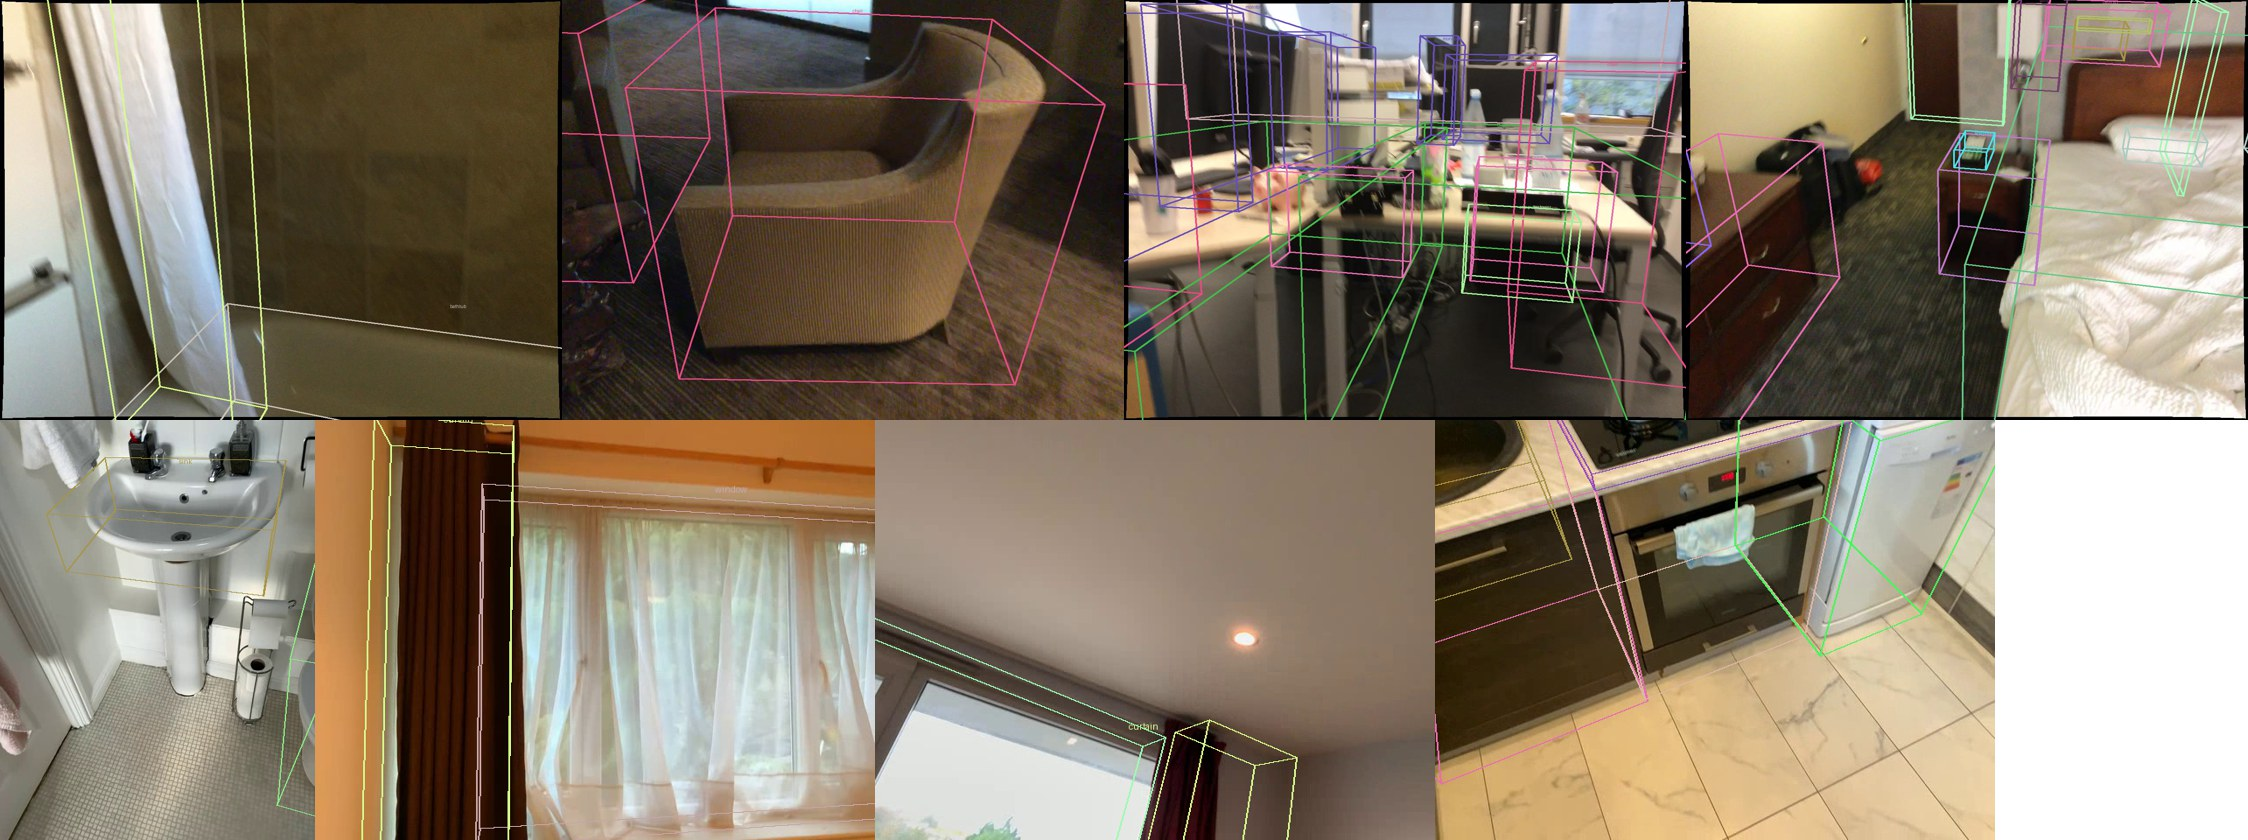
\includegraphics[width=\linewidth]{vggt-det-training-data-overlay.jpg}
\caption{Ground-truth boxes projected into the images with the stored alignment matrix, pose and intrinsics.
Top: ScanNet. Bottom: ARKitScenes after the correction.}
\label{fig:vggtdet-overlay}
\end{figure}

\subsection{Corrections}
\label{sec:vggtdet-data-fix}

\paragraph{Origin.}
For each ARKitScenes scene the alignment matrix gets an extra translation that moves the mean $x$, $y$ of the
points to 0 and their 2nd $z$ percentile (the floor) to 0; the boxes move with it. The median shift is 0.85,
1.87 and 1.23\,m in $x$, $y$ and $z$. The rotation is untouched. Box centres expressed in the scene's world
frame, and hence in every camera's frame, change by less than $10^{-14}$\,m, and sizes do not change.

\paragraph{Focal length.}
Portrait scenes whose focal length is below 0.72 of the long image side (the camera's true value is 0.82 to
0.85) get it multiplied by height over width. This applies to 1,031 of 2,267 training scenes and 265 of 562
validation scenes. Applying either correction a second time changes nothing.

\paragraph{Scope.}
The corrections are applied to the ARKitScenes training and validation files of the 63-class detector and are
built into the two converters that write such files. The files used for inference on Reason-190K and
VSI-Bench keep the first-camera origin on purpose, because the downstream code expects the detections in that
frame. Their portrait focal lengths are still too small; the detector does not read them, but the converter
that writes them (\texttt{build\_arkit\_inputs.py}) should scale by the long image side.
; needs \usepackage{booktabs} and \usepackage{graphicx}.
% Figure file: vggt-det-training-data-overlay.jpg (same folder).
% Data: vggtdet_es56/data/scannet/scannet_infos_train_vsi63.pkl (958 scenes),
%       vggtdet_es56/data/arkit_r190k/arkit_infos_{train,val}_vsi63.pkl (2,267 / 562 scenes).
% Sources: vggtdet_es56/code/tools/vsi63/check_frames_{static,pipeline,model,overlay}.py, scannet_frame.py;
%          results in vggtdet_es56/runs/frame_check/{static,static_after,pipeline,pipeline_after,model}.json.
% Static checks: 150 random scenes per dataset. Pipeline check: 60 random training samples per dataset.

\section{Training data for VGG-T-Det: one box frame for ScanNet and ARKitScenes}
\label{sec:vggtdet-data}

\paragraph{Question.}
VGG-T-Det is fine-tuned on EmbodiedScan boxes of ScanNet (958 scenes) and ARKitScenes (2,267 scenes). The
ScanNet files come from the original VGG-T-Det release, the ARKitScenes files from our own converter. The two
must describe boxes in the same way, or the detector is trained on contradictory targets. We checked this with
several independent tests, each run identically on both datasets so that ScanNet's numbers are the reference.

\paragraph{What the detector's targets depend on.}
The head predicts a box centre in the frame of the first input image and maps it to the scene's aligned frame
with (alignment matrix) $\times$ (pose of the first image). Sizes are predicted directly along the aligned
frame's axes. The targets therefore depend on the rotation of the aligned frame (which way is up, whether the
walls lie on $x$ and $y$), the camera convention of the poses, the metric scale, and the box definition
(gravity centre, axis-aligned size). They do not depend on where the aligned frame's origin is: moving the
origin moves the alignment matrix and the boxes together, and the centre in the first image's frame stays the
same. The stored camera intrinsics are not used by the detector, which takes them from VGGT.

\paragraph{Result.}
The ARKitScenes boxes already agreed with ScanNet in everything the targets depend on. Two things differed,
and neither changed the targets:
\begin{itemize}
\item \textbf{Origin.} ScanNet's aligned frame has the floor at $z=0$ and the mean $x$, $y$ of the scene at 0.
The ARKitScenes files put the origin at the first camera of the trajectory, so the floor was at about
$-1.2$\,m.
\item \textbf{Focal length of portrait videos.} The converter scaled the sensor focal length by image width
over sensor width, which is correct for landscape videos and 0.75 times too small for portrait ones
(398 instead of 531 pixels for a $480\times640$ image). This affected 1,031 of the 2,267 training scenes.
\end{itemize}
Both are now corrected in the ARKitScenes training and validation files (Section~\ref{sec:vggtdet-data-fix}).
Checkpoints trained before the correction remain valid, because the targets are unchanged.

\subsection{Size of the training data}
\label{sec:vggtdet-data-size}

Table~\ref{tab:vggtdet-size} counts the scenes and boxes of the 65-class detector. ScanNet and ARKitScenes use
the EmbodiedScan boxes, ScanNet++ its own annotations. The ARKitScenes and ScanNet++ files include the scenes
built from the raw downloads (\texttt{*\_vsi65\_full.pkl}); before those were added there were 4,272 scenes and
79,670 boxes (ARKitScenes 2,267 / 562 scenes and 39,414 / 9,663 boxes, ScanNet++ 218 / 24 scenes and 7,139 / 742
boxes). Eleven more ARKitScenes training scenes were built but left out (ten with fewer than 42 frames, one without
a box of the 65 classes), and 605 downloaded ScanNet++ scenes lack camera poses. During training ARKitScenes is
validated on a subset of 187 scenes with 3,306 boxes.

\begin{table}[t]
\centering
\caption{Scenes and boxes of the 65-class VGG-T-Det training data (train / validation).}
\label{tab:vggtdet-size}
\begin{tabular}{lrrrrrr}
\toprule
 & \multicolumn{3}{c}{Scenes} & \multicolumn{3}{c}{Boxes} \\
\cmidrule(lr){2-4}\cmidrule(lr){5-7}
Dataset & Train & Val & Total & Train & Val & Total \\
\midrule
ScanNet (EmbodiedScan)     &   958 &   243 & 1,201 & 18,214 &  4,498 &  22,712 \\
ARKitScenes (EmbodiedScan) & 3,587 &   899 & 4,486 & 59,780 & 14,866 &  74,646 \\
ScanNet++                  &   227 &    24 &   251 &  7,543 &    742 &   8,285 \\
\midrule
Total                      & 4,701 & 1,237 & 5,938 & 85,537 & 20,106 & 105,643 \\
\bottomrule
\end{tabular}
\end{table}

\subsection{Checks on the stored files}

\paragraph{Boxes against points.}
Each scene has a point cloud in its raw frame. We move it to the aligned frame and count the points inside each
box. A consistent frame gives full boxes as stored and emptier boxes after any deliberately wrong transform
(Table~\ref{tab:vggtdet-occ}). In both datasets nearly every box holds points as stored, and every wrong
variant loses between a quarter and all of them. For boxes at least twice as long as wide, the points around
the box spread along the box's long side in 98.1\% (ScanNet, 880 boxes) and 97.7\% (ARKitScenes, 745 boxes) of
cases, so $x$ and $y$ sizes are not exchanged.

\begin{table}[t]
\centering
\caption{Boxes against points in the aligned frame (150 scenes per dataset; 2,784 ScanNet and 2,578
ARKitScenes boxes; ARKitScenes after the origin correction). First row: share of boxes holding at least 10
points. Other rows: number of points inside all boxes after a wrong transform, relative to the stored boxes.}
\label{tab:vggtdet-occ}
\begin{tabular}{lrr}
\toprule
 & ScanNet & ARKitScenes \\
\midrule
Boxes with $\geq 10$ points, as stored      & 98.5\% & 99.8\% \\
\midrule
Points not moved to the aligned frame       & 0.05 & 0.12 \\
Boxes turned $90^\circ$ about $z$           & 0.34 & 0.33 \\
Boxes flipped in $z$                        & 0.08 & 0.00 \\
Centre read as bottom of the box            & 0.66 & 0.78 \\
Centre read as top of the box               & 0.58 & 0.55 \\
$x$ and $y$ sizes exchanged                 & 0.59 & 0.64 \\
\bottomrule
\end{tabular}
\end{table}

\paragraph{Up direction, walls, cameras.}
Table~\ref{tab:vggtdet-frame} lists the remaining properties of the frame. In both datasets $z$ is up, the
images are upright, the cameras are about 1.4 to 1.5\,m above the floor, and the walls lie on $x$ and $y$. The
wall test turns the point cloud about $z$ and looks for the turn that makes the $x$ and $y$ histograms
sharpest; this turn is within $3^\circ$ of zero in 97\% and 94\% of scenes.

\paragraph{Camera convention.}
We project the coloured points into the images with the stored pose and intrinsics, keep the nearest point
per $8\times8$ pixel cell, and correlate point and image brightness. The stored convention (camera-to-world,
OpenCV axes) gives 0.71 on ScanNet and 0.74 on ARKitScenes; an OpenGL camera or an inverted pose gives about
zero on both. This test found the focal-length error: portrait ARKitScenes images scored 0.41 as stored and
0.77 with the focal length multiplied by $4/3$, while landscape images scored 0.71 as stored.

\begin{table}[t]
\centering
\caption{Frame properties (150 scenes per dataset). ARKitScenes values that changed with the correction are
given as before $\rightarrow$ after.}
\label{tab:vggtdet-frame}
\begin{tabular}{lrr}
\toprule
 & ScanNet & ARKitScenes \\
\midrule
Image-up direction, mean $z$ component          & 0.88 & 0.84 \\
Scenes with upright images                       & 100\% & 100\% \\
Frames rolled by more than $45^\circ$            & 0.02\% & 0.07\% \\
Camera height above the floor (median)           & 1.38\,m & 1.48\,m \\
Walls within $3^\circ$ of $x$ / $y$              & 97\% & 94\% \\
Brightness correlation, stored camera            & 0.71 & 0.51 $\rightarrow$ 0.74 \\
Brightness correlation, OpenGL camera            & $-0.01$ & $-0.01$ \\
Brightness correlation, inverted pose            & 0.15 & 0.00 \\
Floor height in the aligned frame (median)       & $-0.04$\,m & $-1.22 \rightarrow 0.00$\,m \\
\bottomrule
\end{tabular}
\end{table}

\paragraph{Sizes per class.}
For the 18 classes with at least 30 boxes in both samples, the per-class medians agree between the datasets:
the correlation over classes is 0.93 for height, 0.84 for the long side, 0.97 for the short side and 0.95 for
the centre height above the floor. Height in one dataset against the long side in the other gives 0.30. The
scale is metric in both and the vertical axis is the same.

\subsection{Check on what the model receives}

The same tests were run on samples taken from the real training pipeline, after the step that turns the
aligned frame so that $+y$ is the wall direction nearest the first image's viewing direction
(60 samples per dataset; 1,116 ScanNet and 1,047 ARKitScenes boxes). The points arrive in the first image's
frame and the boxes in the aligned frame; we applied the matrix the head uses to the points. With it, 98.1\%
(ScanNet) and 99.9\% (ARKitScenes) of boxes hold at least 10 points; leaving out either the pose or the
alignment matrix leaves 4--10\% of the points inside the boxes. The first image looks within $45^\circ$ of
$+y$ in every sample of both datasets (median $17^\circ$ and $16^\circ$ off). The box centres seen from the
first image have similar ranges in both datasets, and for ARKitScenes they are identical before and after the
origin correction.

\subsection{Check with a detector trained on ScanNet only}

A detector that has only seen ScanNet carries ScanNet's box convention. If the ARKitScenes frame agrees, its
boxes on ARKitScenes must land on the ARKitScenes ground truth, and wrong transforms of its boxes must destroy
the overlap just as they do on ScanNet. Table~\ref{tab:vggtdet-model} shows this. The overlap on ARKitScenes
is lower, as expected for an unseen dataset, but a quarter turn, a flip in $z$, or reading the centre as the
bottom or top of the box reduces it in the same way.

\begin{table}[t]
\centering
\caption{Mean IoU between boxes of the ScanNet-only detector (score $\geq 0.3$) and the nearest ground-truth
box of the same class (15,163 pairs on ScanNet, 10,500 on ARKitScenes), as predicted and after wrong
transforms of the predictions.}
\label{tab:vggtdet-model}
\begin{tabular}{lrr}
\toprule
 & ScanNet & ARKitScenes \\
\midrule
As predicted                         & 0.41 & 0.21 \\
Turned $90^\circ$ about $z$          & 0.01 & 0.00 \\
Flipped in $z$                       & 0.01 & 0.04 \\
Centre read as bottom of the box     & 0.19 & 0.13 \\
Centre read as top of the box        & 0.18 & 0.10 \\
\bottomrule
\end{tabular}
\end{table}

\paragraph{An offset that is not a frame error.}
On ARKitScenes the ScanNet-only detector places its boxes a median of 0.16\,m too far along the first image's
viewing direction (ScanNet: 0.01\,m). The offset is constant with distance (slope 1.01), so it is not a scale
error. To decide whether the ground truth or the model is off, we moved the stored camera position in steps of
5\,cm along its three axes and repeated the brightness test. On both datasets the correlation is highest at
zero shift in all three directions (ScanNet 0.64, ARKitScenes 0.63, about 350 images each) and falls on either
side. The stored poses, images and points therefore agree, and the offset is a bias of the ScanNet-trained
model on ARKitScenes images, which fine-tuning on ARKitScenes is meant to remove.

\subsection{Visual check}

Figure~\ref{fig:vggtdet-overlay} draws the stored boxes into the images. The boxes sit on the objects in both
datasets, including portrait ARKitScenes images with the corrected focal length.

\begin{figure}[t]
\centering
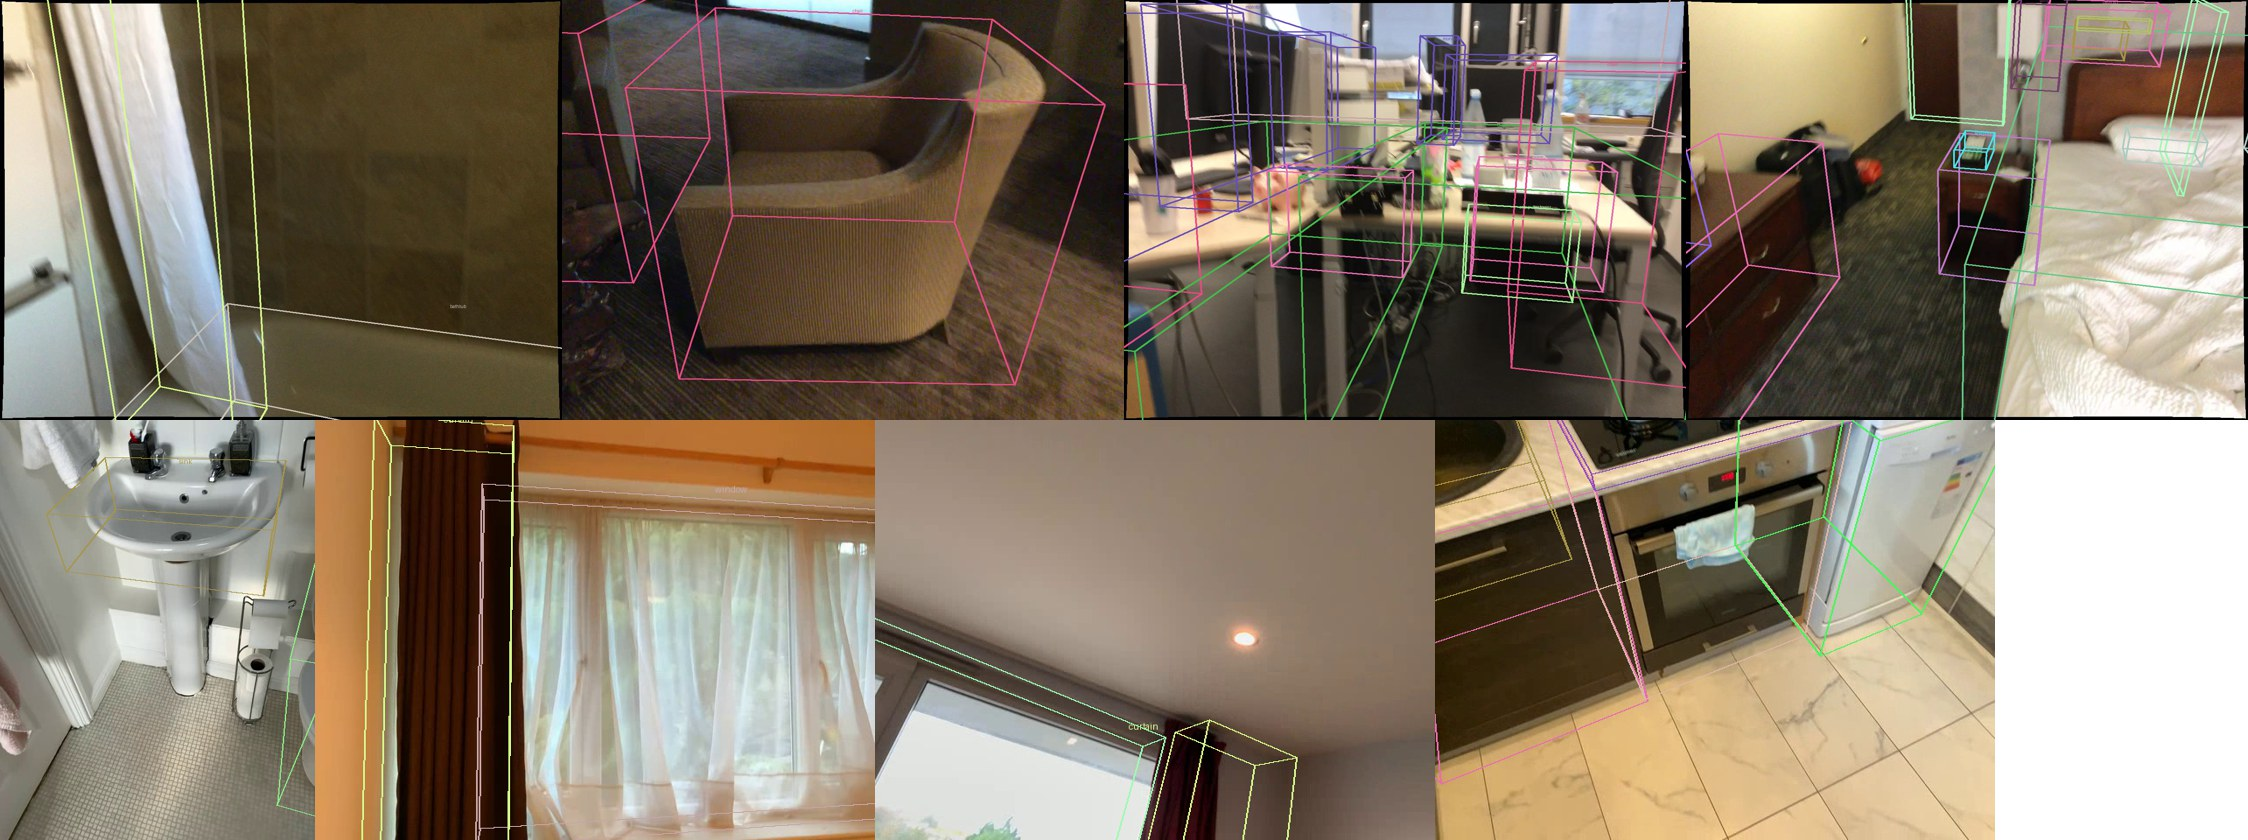
\includegraphics[width=\linewidth]{vggt-det-training-data-overlay.jpg}
\caption{Ground-truth boxes projected into the images with the stored alignment matrix, pose and intrinsics.
Top: ScanNet. Bottom: ARKitScenes after the correction.}
\label{fig:vggtdet-overlay}
\end{figure}

\subsection{Corrections}
\label{sec:vggtdet-data-fix}

\paragraph{Origin.}
For each ARKitScenes scene the alignment matrix gets an extra translation that moves the mean $x$, $y$ of the
points to 0 and their 2nd $z$ percentile (the floor) to 0; the boxes move with it. The median shift is 0.85,
1.87 and 1.23\,m in $x$, $y$ and $z$. The rotation is untouched. Box centres expressed in the scene's world
frame, and hence in every camera's frame, change by less than $10^{-14}$\,m, and sizes do not change.

\paragraph{Focal length.}
Portrait scenes whose focal length is below 0.72 of the long image side (the camera's true value is 0.82 to
0.85) get it multiplied by height over width. This applies to 1,031 of 2,267 training scenes and 265 of 562
validation scenes. Applying either correction a second time changes nothing.

\paragraph{Scope.}
The corrections are applied to the ARKitScenes training and validation files of the 63-class detector and are
built into the two converters that write such files. The files used for inference on Reason-190K and
VSI-Bench keep the first-camera origin on purpose, because the downstream code expects the detections in that
frame. Their portrait focal lengths are still too small; the detector does not read them, but the converter
that writes them (\texttt{build\_arkit\_inputs.py}) should scale by the long image side.
; needs \usepackage{booktabs} and \usepackage{graphicx}.
% Figure file: vggt-det-training-data-overlay.jpg (same folder).
% Data: vggtdet_es56/data/scannet/scannet_infos_train_vsi63.pkl (958 scenes),
%       vggtdet_es56/data/arkit_r190k/arkit_infos_{train,val}_vsi63.pkl (2,267 / 562 scenes).
% Sources: vggtdet_es56/code/tools/vsi63/check_frames_{static,pipeline,model,overlay}.py, scannet_frame.py;
%          results in vggtdet_es56/runs/frame_check/{static,static_after,pipeline,pipeline_after,model}.json.
% Static checks: 150 random scenes per dataset. Pipeline check: 60 random training samples per dataset.

\section{Training data for VGG-T-Det: one box frame for ScanNet and ARKitScenes}
\label{sec:vggtdet-data}

\paragraph{Question.}
VGG-T-Det is fine-tuned on EmbodiedScan boxes of ScanNet (958 scenes) and ARKitScenes (2,267 scenes). The
ScanNet files come from the original VGG-T-Det release, the ARKitScenes files from our own converter. The two
must describe boxes in the same way, or the detector is trained on contradictory targets. We checked this with
several independent tests, each run identically on both datasets so that ScanNet's numbers are the reference.

\paragraph{What the detector's targets depend on.}
The head predicts a box centre in the frame of the first input image and maps it to the scene's aligned frame
with (alignment matrix) $\times$ (pose of the first image). Sizes are predicted directly along the aligned
frame's axes. The targets therefore depend on the rotation of the aligned frame (which way is up, whether the
walls lie on $x$ and $y$), the camera convention of the poses, the metric scale, and the box definition
(gravity centre, axis-aligned size). They do not depend on where the aligned frame's origin is: moving the
origin moves the alignment matrix and the boxes together, and the centre in the first image's frame stays the
same. The stored camera intrinsics are not used by the detector, which takes them from VGGT.

\paragraph{Result.}
The ARKitScenes boxes already agreed with ScanNet in everything the targets depend on. Two things differed,
and neither changed the targets:
\begin{itemize}
\item \textbf{Origin.} ScanNet's aligned frame has the floor at $z=0$ and the mean $x$, $y$ of the scene at 0.
The ARKitScenes files put the origin at the first camera of the trajectory, so the floor was at about
$-1.2$\,m.
\item \textbf{Focal length of portrait videos.} The converter scaled the sensor focal length by image width
over sensor width, which is correct for landscape videos and 0.75 times too small for portrait ones
(398 instead of 531 pixels for a $480\times640$ image). This affected 1,031 of the 2,267 training scenes.
\end{itemize}
Both are now corrected in the ARKitScenes training and validation files (Section~\ref{sec:vggtdet-data-fix}).
Checkpoints trained before the correction remain valid, because the targets are unchanged.

\subsection{Size of the training data}
\label{sec:vggtdet-data-size}

Table~\ref{tab:vggtdet-size} counts the scenes and boxes of the 65-class detector. ScanNet and ARKitScenes use
the EmbodiedScan boxes, ScanNet++ its own annotations. The ARKitScenes and ScanNet++ files include the scenes
built from the raw downloads (\texttt{*\_vsi65\_full.pkl}); before those were added there were 4,272 scenes and
79,670 boxes (ARKitScenes 2,267 / 562 scenes and 39,414 / 9,663 boxes, ScanNet++ 218 / 24 scenes and 7,139 / 742
boxes). Eleven more ARKitScenes training scenes were built but left out (ten with fewer than 42 frames, one without
a box of the 65 classes), and 605 downloaded ScanNet++ scenes lack camera poses. During training ARKitScenes is
validated on a subset of 187 scenes with 3,306 boxes.

\begin{table}[t]
\centering
\caption{Scenes and boxes of the 65-class VGG-T-Det training data (train / validation).}
\label{tab:vggtdet-size}
\begin{tabular}{lrrrrrr}
\toprule
 & \multicolumn{3}{c}{Scenes} & \multicolumn{3}{c}{Boxes} \\
\cmidrule(lr){2-4}\cmidrule(lr){5-7}
Dataset & Train & Val & Total & Train & Val & Total \\
\midrule
ScanNet (EmbodiedScan)     &   958 &   243 & 1,201 & 18,214 &  4,498 &  22,712 \\
ARKitScenes (EmbodiedScan) & 3,587 &   899 & 4,486 & 59,780 & 14,866 &  74,646 \\
ScanNet++                  &   227 &    24 &   251 &  7,543 &    742 &   8,285 \\
\midrule
Total                      & 4,701 & 1,237 & 5,938 & 85,537 & 20,106 & 105,643 \\
\bottomrule
\end{tabular}
\end{table}

\subsection{Checks on the stored files}

\paragraph{Boxes against points.}
Each scene has a point cloud in its raw frame. We move it to the aligned frame and count the points inside each
box. A consistent frame gives full boxes as stored and emptier boxes after any deliberately wrong transform
(Table~\ref{tab:vggtdet-occ}). In both datasets nearly every box holds points as stored, and every wrong
variant loses between a quarter and all of them. For boxes at least twice as long as wide, the points around
the box spread along the box's long side in 98.1\% (ScanNet, 880 boxes) and 97.7\% (ARKitScenes, 745 boxes) of
cases, so $x$ and $y$ sizes are not exchanged.

\begin{table}[t]
\centering
\caption{Boxes against points in the aligned frame (150 scenes per dataset; 2,784 ScanNet and 2,578
ARKitScenes boxes; ARKitScenes after the origin correction). First row: share of boxes holding at least 10
points. Other rows: number of points inside all boxes after a wrong transform, relative to the stored boxes.}
\label{tab:vggtdet-occ}
\begin{tabular}{lrr}
\toprule
 & ScanNet & ARKitScenes \\
\midrule
Boxes with $\geq 10$ points, as stored      & 98.5\% & 99.8\% \\
\midrule
Points not moved to the aligned frame       & 0.05 & 0.12 \\
Boxes turned $90^\circ$ about $z$           & 0.34 & 0.33 \\
Boxes flipped in $z$                        & 0.08 & 0.00 \\
Centre read as bottom of the box            & 0.66 & 0.78 \\
Centre read as top of the box               & 0.58 & 0.55 \\
$x$ and $y$ sizes exchanged                 & 0.59 & 0.64 \\
\bottomrule
\end{tabular}
\end{table}

\paragraph{Up direction, walls, cameras.}
Table~\ref{tab:vggtdet-frame} lists the remaining properties of the frame. In both datasets $z$ is up, the
images are upright, the cameras are about 1.4 to 1.5\,m above the floor, and the walls lie on $x$ and $y$. The
wall test turns the point cloud about $z$ and looks for the turn that makes the $x$ and $y$ histograms
sharpest; this turn is within $3^\circ$ of zero in 97\% and 94\% of scenes.

\paragraph{Camera convention.}
We project the coloured points into the images with the stored pose and intrinsics, keep the nearest point
per $8\times8$ pixel cell, and correlate point and image brightness. The stored convention (camera-to-world,
OpenCV axes) gives 0.71 on ScanNet and 0.74 on ARKitScenes; an OpenGL camera or an inverted pose gives about
zero on both. This test found the focal-length error: portrait ARKitScenes images scored 0.41 as stored and
0.77 with the focal length multiplied by $4/3$, while landscape images scored 0.71 as stored.

\begin{table}[t]
\centering
\caption{Frame properties (150 scenes per dataset). ARKitScenes values that changed with the correction are
given as before $\rightarrow$ after.}
\label{tab:vggtdet-frame}
\begin{tabular}{lrr}
\toprule
 & ScanNet & ARKitScenes \\
\midrule
Image-up direction, mean $z$ component          & 0.88 & 0.84 \\
Scenes with upright images                       & 100\% & 100\% \\
Frames rolled by more than $45^\circ$            & 0.02\% & 0.07\% \\
Camera height above the floor (median)           & 1.38\,m & 1.48\,m \\
Walls within $3^\circ$ of $x$ / $y$              & 97\% & 94\% \\
Brightness correlation, stored camera            & 0.71 & 0.51 $\rightarrow$ 0.74 \\
Brightness correlation, OpenGL camera            & $-0.01$ & $-0.01$ \\
Brightness correlation, inverted pose            & 0.15 & 0.00 \\
Floor height in the aligned frame (median)       & $-0.04$\,m & $-1.22 \rightarrow 0.00$\,m \\
\bottomrule
\end{tabular}
\end{table}

\paragraph{Sizes per class.}
For the 18 classes with at least 30 boxes in both samples, the per-class medians agree between the datasets:
the correlation over classes is 0.93 for height, 0.84 for the long side, 0.97 for the short side and 0.95 for
the centre height above the floor. Height in one dataset against the long side in the other gives 0.30. The
scale is metric in both and the vertical axis is the same.

\subsection{Check on what the model receives}

The same tests were run on samples taken from the real training pipeline, after the step that turns the
aligned frame so that $+y$ is the wall direction nearest the first image's viewing direction
(60 samples per dataset; 1,116 ScanNet and 1,047 ARKitScenes boxes). The points arrive in the first image's
frame and the boxes in the aligned frame; we applied the matrix the head uses to the points. With it, 98.1\%
(ScanNet) and 99.9\% (ARKitScenes) of boxes hold at least 10 points; leaving out either the pose or the
alignment matrix leaves 4--10\% of the points inside the boxes. The first image looks within $45^\circ$ of
$+y$ in every sample of both datasets (median $17^\circ$ and $16^\circ$ off). The box centres seen from the
first image have similar ranges in both datasets, and for ARKitScenes they are identical before and after the
origin correction.

\subsection{Check with a detector trained on ScanNet only}

A detector that has only seen ScanNet carries ScanNet's box convention. If the ARKitScenes frame agrees, its
boxes on ARKitScenes must land on the ARKitScenes ground truth, and wrong transforms of its boxes must destroy
the overlap just as they do on ScanNet. Table~\ref{tab:vggtdet-model} shows this. The overlap on ARKitScenes
is lower, as expected for an unseen dataset, but a quarter turn, a flip in $z$, or reading the centre as the
bottom or top of the box reduces it in the same way.

\begin{table}[t]
\centering
\caption{Mean IoU between boxes of the ScanNet-only detector (score $\geq 0.3$) and the nearest ground-truth
box of the same class (15,163 pairs on ScanNet, 10,500 on ARKitScenes), as predicted and after wrong
transforms of the predictions.}
\label{tab:vggtdet-model}
\begin{tabular}{lrr}
\toprule
 & ScanNet & ARKitScenes \\
\midrule
As predicted                         & 0.41 & 0.21 \\
Turned $90^\circ$ about $z$          & 0.01 & 0.00 \\
Flipped in $z$                       & 0.01 & 0.04 \\
Centre read as bottom of the box     & 0.19 & 0.13 \\
Centre read as top of the box        & 0.18 & 0.10 \\
\bottomrule
\end{tabular}
\end{table}

\paragraph{An offset that is not a frame error.}
On ARKitScenes the ScanNet-only detector places its boxes a median of 0.16\,m too far along the first image's
viewing direction (ScanNet: 0.01\,m). The offset is constant with distance (slope 1.01), so it is not a scale
error. To decide whether the ground truth or the model is off, we moved the stored camera position in steps of
5\,cm along its three axes and repeated the brightness test. On both datasets the correlation is highest at
zero shift in all three directions (ScanNet 0.64, ARKitScenes 0.63, about 350 images each) and falls on either
side. The stored poses, images and points therefore agree, and the offset is a bias of the ScanNet-trained
model on ARKitScenes images, which fine-tuning on ARKitScenes is meant to remove.

\subsection{Visual check}

Figure~\ref{fig:vggtdet-overlay} draws the stored boxes into the images. The boxes sit on the objects in both
datasets, including portrait ARKitScenes images with the corrected focal length.

\begin{figure}[t]
\centering
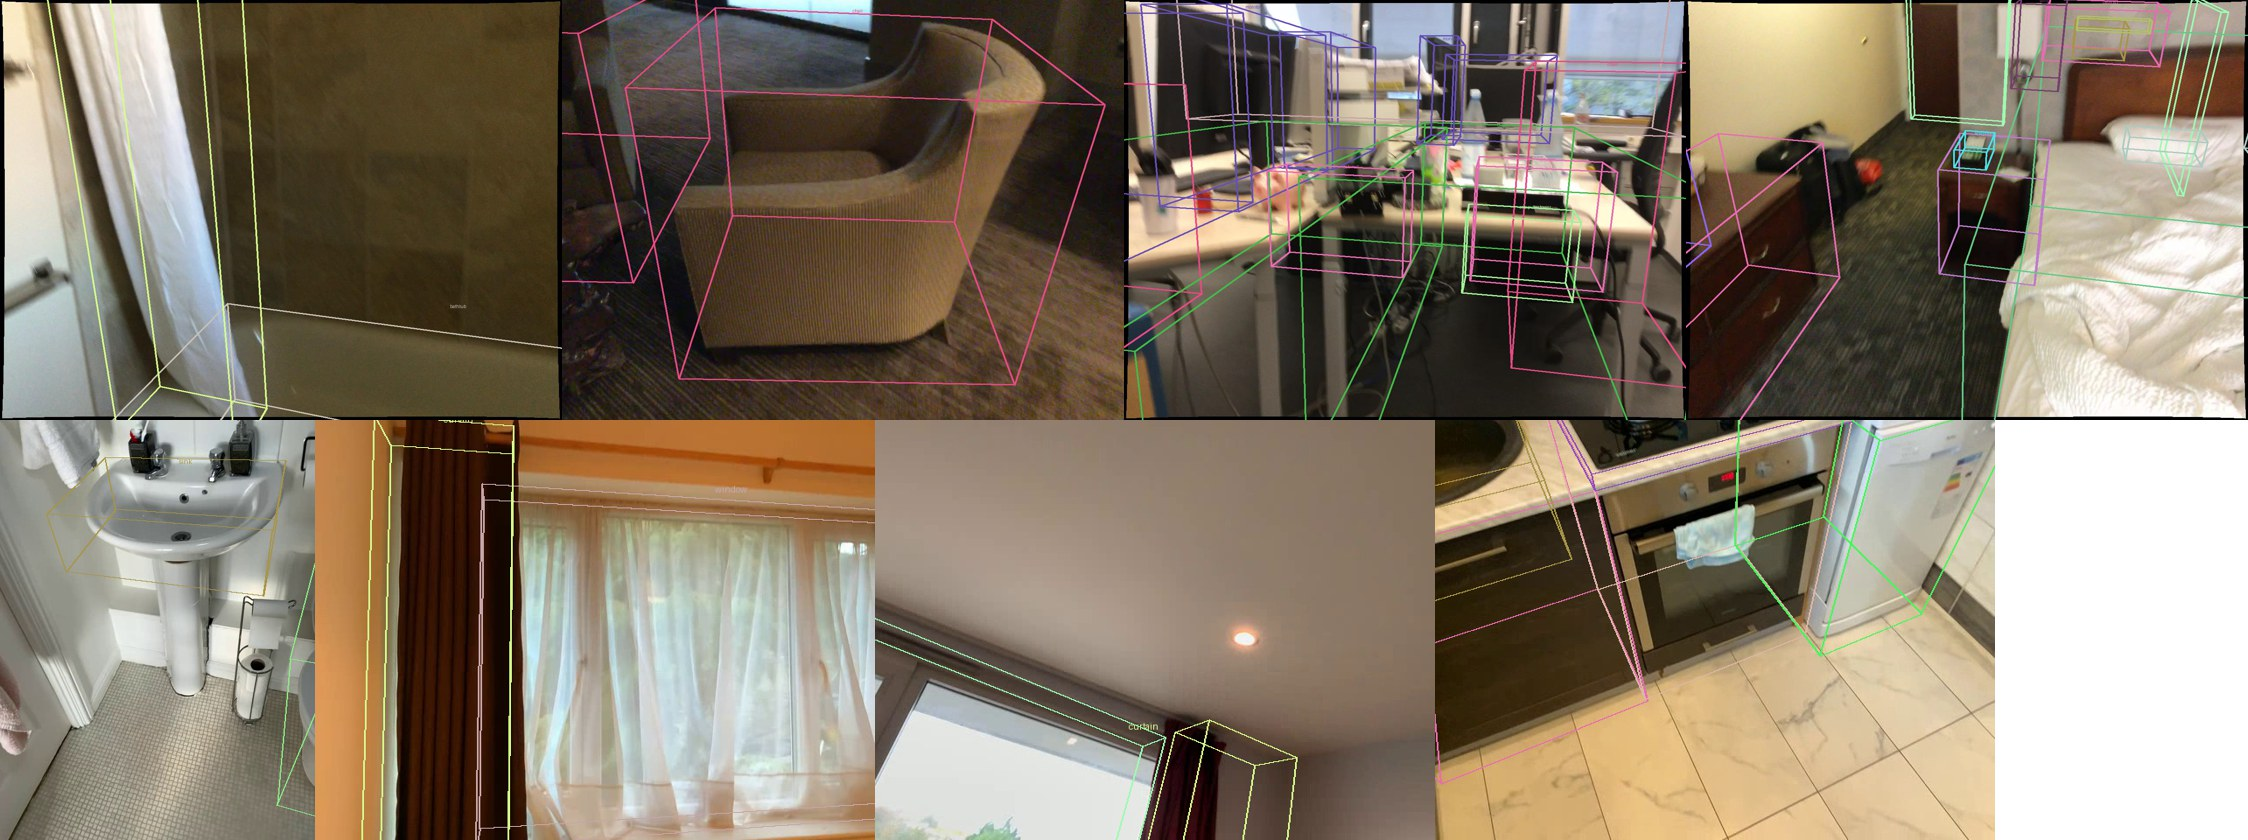
\includegraphics[width=\linewidth]{vggt-det-training-data-overlay.jpg}
\caption{Ground-truth boxes projected into the images with the stored alignment matrix, pose and intrinsics.
Top: ScanNet. Bottom: ARKitScenes after the correction.}
\label{fig:vggtdet-overlay}
\end{figure}

\subsection{Corrections}
\label{sec:vggtdet-data-fix}

\paragraph{Origin.}
For each ARKitScenes scene the alignment matrix gets an extra translation that moves the mean $x$, $y$ of the
points to 0 and their 2nd $z$ percentile (the floor) to 0; the boxes move with it. The median shift is 0.85,
1.87 and 1.23\,m in $x$, $y$ and $z$. The rotation is untouched. Box centres expressed in the scene's world
frame, and hence in every camera's frame, change by less than $10^{-14}$\,m, and sizes do not change.

\paragraph{Focal length.}
Portrait scenes whose focal length is below 0.72 of the long image side (the camera's true value is 0.82 to
0.85) get it multiplied by height over width. This applies to 1,031 of 2,267 training scenes and 265 of 562
validation scenes. Applying either correction a second time changes nothing.

\paragraph{Scope.}
The corrections are applied to the ARKitScenes training and validation files of the 63-class detector and are
built into the two converters that write such files. The files used for inference on Reason-190K and
VSI-Bench keep the first-camera origin on purpose, because the downstream code expects the detections in that
frame. Their portrait focal lengths are still too small; the detector does not read them, but the converter
that writes them (\texttt{build\_arkit\_inputs.py}) should scale by the long image side.
; needs \usepackage{booktabs} and \usepackage{graphicx}.
% Figure file: vggt-det-training-data-overlay.jpg (same folder).
% Data: vggtdet_es56/data/scannet/scannet_infos_train_vsi63.pkl (958 scenes),
%       vggtdet_es56/data/arkit_r190k/arkit_infos_{train,val}_vsi63.pkl (2,267 / 562 scenes).
% Sources: vggtdet_es56/code/tools/vsi63/check_frames_{static,pipeline,model,overlay}.py, scannet_frame.py;
%          results in vggtdet_es56/runs/frame_check/{static,static_after,pipeline,pipeline_after,model}.json.
% Static checks: 150 random scenes per dataset. Pipeline check: 60 random training samples per dataset.

\section{Training data for VGG-T-Det: one box frame for ScanNet and ARKitScenes}
\label{sec:vggtdet-data}

\paragraph{Question.}
VGG-T-Det is fine-tuned on EmbodiedScan boxes of ScanNet (958 scenes) and ARKitScenes (2,267 scenes). The
ScanNet files come from the original VGG-T-Det release, the ARKitScenes files from our own converter. The two
must describe boxes in the same way, or the detector is trained on contradictory targets. We checked this with
several independent tests, each run identically on both datasets so that ScanNet's numbers are the reference.

\paragraph{What the detector's targets depend on.}
The head predicts a box centre in the frame of the first input image and maps it to the scene's aligned frame
with (alignment matrix) $\times$ (pose of the first image). Sizes are predicted directly along the aligned
frame's axes. The targets therefore depend on the rotation of the aligned frame (which way is up, whether the
walls lie on $x$ and $y$), the camera convention of the poses, the metric scale, and the box definition
(gravity centre, axis-aligned size). They do not depend on where the aligned frame's origin is: moving the
origin moves the alignment matrix and the boxes together, and the centre in the first image's frame stays the
same. The stored camera intrinsics are not used by the detector, which takes them from VGGT.

\paragraph{Result.}
The ARKitScenes boxes already agreed with ScanNet in everything the targets depend on. Two things differed,
and neither changed the targets:
\begin{itemize}
\item \textbf{Origin.} ScanNet's aligned frame has the floor at $z=0$ and the mean $x$, $y$ of the scene at 0.
The ARKitScenes files put the origin at the first camera of the trajectory, so the floor was at about
$-1.2$\,m.
\item \textbf{Focal length of portrait videos.} The converter scaled the sensor focal length by image width
over sensor width, which is correct for landscape videos and 0.75 times too small for portrait ones
(398 instead of 531 pixels for a $480\times640$ image). This affected 1,031 of the 2,267 training scenes.
\end{itemize}
Both are now corrected in the ARKitScenes training and validation files (Section~\ref{sec:vggtdet-data-fix}).
Checkpoints trained before the correction remain valid, because the targets are unchanged.

\subsection{Size of the training data}
\label{sec:vggtdet-data-size}

Table~\ref{tab:vggtdet-size} counts the scenes and boxes of the 65-class detector. ScanNet and ARKitScenes use
the EmbodiedScan boxes, ScanNet++ its own annotations. The ARKitScenes and ScanNet++ files include the scenes
built from the raw downloads (\texttt{*\_vsi65\_full.pkl}); before those were added there were 4,272 scenes and
79,670 boxes (ARKitScenes 2,267 / 562 scenes and 39,414 / 9,663 boxes, ScanNet++ 218 / 24 scenes and 7,139 / 742
boxes). Eleven more ARKitScenes training scenes were built but left out (ten with fewer than 42 frames, one without
a box of the 65 classes), and 605 downloaded ScanNet++ scenes lack camera poses. During training ARKitScenes is
validated on a subset of 187 scenes with 3,306 boxes.

\begin{table}[t]
\centering
\caption{Scenes and boxes of the 65-class VGG-T-Det training data (train / validation).}
\label{tab:vggtdet-size}
\begin{tabular}{lrrrrrr}
\toprule
 & \multicolumn{3}{c}{Scenes} & \multicolumn{3}{c}{Boxes} \\
\cmidrule(lr){2-4}\cmidrule(lr){5-7}
Dataset & Train & Val & Total & Train & Val & Total \\
\midrule
ScanNet (EmbodiedScan)     &   958 &   243 & 1,201 & 18,214 &  4,498 &  22,712 \\
ARKitScenes (EmbodiedScan) & 3,587 &   899 & 4,486 & 59,780 & 14,866 &  74,646 \\
ScanNet++                  &   227 &    24 &   251 &  7,543 &    742 &   8,285 \\
\midrule
Total                      & 4,701 & 1,237 & 5,938 & 85,537 & 20,106 & 105,643 \\
\bottomrule
\end{tabular}
\end{table}

\subsection{Checks on the stored files}

\paragraph{Boxes against points.}
Each scene has a point cloud in its raw frame. We move it to the aligned frame and count the points inside each
box. A consistent frame gives full boxes as stored and emptier boxes after any deliberately wrong transform
(Table~\ref{tab:vggtdet-occ}). In both datasets nearly every box holds points as stored, and every wrong
variant loses between a quarter and all of them. For boxes at least twice as long as wide, the points around
the box spread along the box's long side in 98.1\% (ScanNet, 880 boxes) and 97.7\% (ARKitScenes, 745 boxes) of
cases, so $x$ and $y$ sizes are not exchanged.

\begin{table}[t]
\centering
\caption{Boxes against points in the aligned frame (150 scenes per dataset; 2,784 ScanNet and 2,578
ARKitScenes boxes; ARKitScenes after the origin correction). First row: share of boxes holding at least 10
points. Other rows: number of points inside all boxes after a wrong transform, relative to the stored boxes.}
\label{tab:vggtdet-occ}
\begin{tabular}{lrr}
\toprule
 & ScanNet & ARKitScenes \\
\midrule
Boxes with $\geq 10$ points, as stored      & 98.5\% & 99.8\% \\
\midrule
Points not moved to the aligned frame       & 0.05 & 0.12 \\
Boxes turned $90^\circ$ about $z$           & 0.34 & 0.33 \\
Boxes flipped in $z$                        & 0.08 & 0.00 \\
Centre read as bottom of the box            & 0.66 & 0.78 \\
Centre read as top of the box               & 0.58 & 0.55 \\
$x$ and $y$ sizes exchanged                 & 0.59 & 0.64 \\
\bottomrule
\end{tabular}
\end{table}

\paragraph{Up direction, walls, cameras.}
Table~\ref{tab:vggtdet-frame} lists the remaining properties of the frame. In both datasets $z$ is up, the
images are upright, the cameras are about 1.4 to 1.5\,m above the floor, and the walls lie on $x$ and $y$. The
wall test turns the point cloud about $z$ and looks for the turn that makes the $x$ and $y$ histograms
sharpest; this turn is within $3^\circ$ of zero in 97\% and 94\% of scenes.

\paragraph{Camera convention.}
We project the coloured points into the images with the stored pose and intrinsics, keep the nearest point
per $8\times8$ pixel cell, and correlate point and image brightness. The stored convention (camera-to-world,
OpenCV axes) gives 0.71 on ScanNet and 0.74 on ARKitScenes; an OpenGL camera or an inverted pose gives about
zero on both. This test found the focal-length error: portrait ARKitScenes images scored 0.41 as stored and
0.77 with the focal length multiplied by $4/3$, while landscape images scored 0.71 as stored.

\begin{table}[t]
\centering
\caption{Frame properties (150 scenes per dataset). ARKitScenes values that changed with the correction are
given as before $\rightarrow$ after.}
\label{tab:vggtdet-frame}
\begin{tabular}{lrr}
\toprule
 & ScanNet & ARKitScenes \\
\midrule
Image-up direction, mean $z$ component          & 0.88 & 0.84 \\
Scenes with upright images                       & 100\% & 100\% \\
Frames rolled by more than $45^\circ$            & 0.02\% & 0.07\% \\
Camera height above the floor (median)           & 1.38\,m & 1.48\,m \\
Walls within $3^\circ$ of $x$ / $y$              & 97\% & 94\% \\
Brightness correlation, stored camera            & 0.71 & 0.51 $\rightarrow$ 0.74 \\
Brightness correlation, OpenGL camera            & $-0.01$ & $-0.01$ \\
Brightness correlation, inverted pose            & 0.15 & 0.00 \\
Floor height in the aligned frame (median)       & $-0.04$\,m & $-1.22 \rightarrow 0.00$\,m \\
\bottomrule
\end{tabular}
\end{table}

\paragraph{Sizes per class.}
For the 18 classes with at least 30 boxes in both samples, the per-class medians agree between the datasets:
the correlation over classes is 0.93 for height, 0.84 for the long side, 0.97 for the short side and 0.95 for
the centre height above the floor. Height in one dataset against the long side in the other gives 0.30. The
scale is metric in both and the vertical axis is the same.

\subsection{Check on what the model receives}

The same tests were run on samples taken from the real training pipeline, after the step that turns the
aligned frame so that $+y$ is the wall direction nearest the first image's viewing direction
(60 samples per dataset; 1,116 ScanNet and 1,047 ARKitScenes boxes). The points arrive in the first image's
frame and the boxes in the aligned frame; we applied the matrix the head uses to the points. With it, 98.1\%
(ScanNet) and 99.9\% (ARKitScenes) of boxes hold at least 10 points; leaving out either the pose or the
alignment matrix leaves 4--10\% of the points inside the boxes. The first image looks within $45^\circ$ of
$+y$ in every sample of both datasets (median $17^\circ$ and $16^\circ$ off). The box centres seen from the
first image have similar ranges in both datasets, and for ARKitScenes they are identical before and after the
origin correction.

\subsection{Check with a detector trained on ScanNet only}

A detector that has only seen ScanNet carries ScanNet's box convention. If the ARKitScenes frame agrees, its
boxes on ARKitScenes must land on the ARKitScenes ground truth, and wrong transforms of its boxes must destroy
the overlap just as they do on ScanNet. Table~\ref{tab:vggtdet-model} shows this. The overlap on ARKitScenes
is lower, as expected for an unseen dataset, but a quarter turn, a flip in $z$, or reading the centre as the
bottom or top of the box reduces it in the same way.

\begin{table}[t]
\centering
\caption{Mean IoU between boxes of the ScanNet-only detector (score $\geq 0.3$) and the nearest ground-truth
box of the same class (15,163 pairs on ScanNet, 10,500 on ARKitScenes), as predicted and after wrong
transforms of the predictions.}
\label{tab:vggtdet-model}
\begin{tabular}{lrr}
\toprule
 & ScanNet & ARKitScenes \\
\midrule
As predicted                         & 0.41 & 0.21 \\
Turned $90^\circ$ about $z$          & 0.01 & 0.00 \\
Flipped in $z$                       & 0.01 & 0.04 \\
Centre read as bottom of the box     & 0.19 & 0.13 \\
Centre read as top of the box        & 0.18 & 0.10 \\
\bottomrule
\end{tabular}
\end{table}

\paragraph{An offset that is not a frame error.}
On ARKitScenes the ScanNet-only detector places its boxes a median of 0.16\,m too far along the first image's
viewing direction (ScanNet: 0.01\,m). The offset is constant with distance (slope 1.01), so it is not a scale
error. To decide whether the ground truth or the model is off, we moved the stored camera position in steps of
5\,cm along its three axes and repeated the brightness test. On both datasets the correlation is highest at
zero shift in all three directions (ScanNet 0.64, ARKitScenes 0.63, about 350 images each) and falls on either
side. The stored poses, images and points therefore agree, and the offset is a bias of the ScanNet-trained
model on ARKitScenes images, which fine-tuning on ARKitScenes is meant to remove.

\subsection{Visual check}

Figure~\ref{fig:vggtdet-overlay} draws the stored boxes into the images. The boxes sit on the objects in both
datasets, including portrait ARKitScenes images with the corrected focal length.

\begin{figure}[t]
\centering
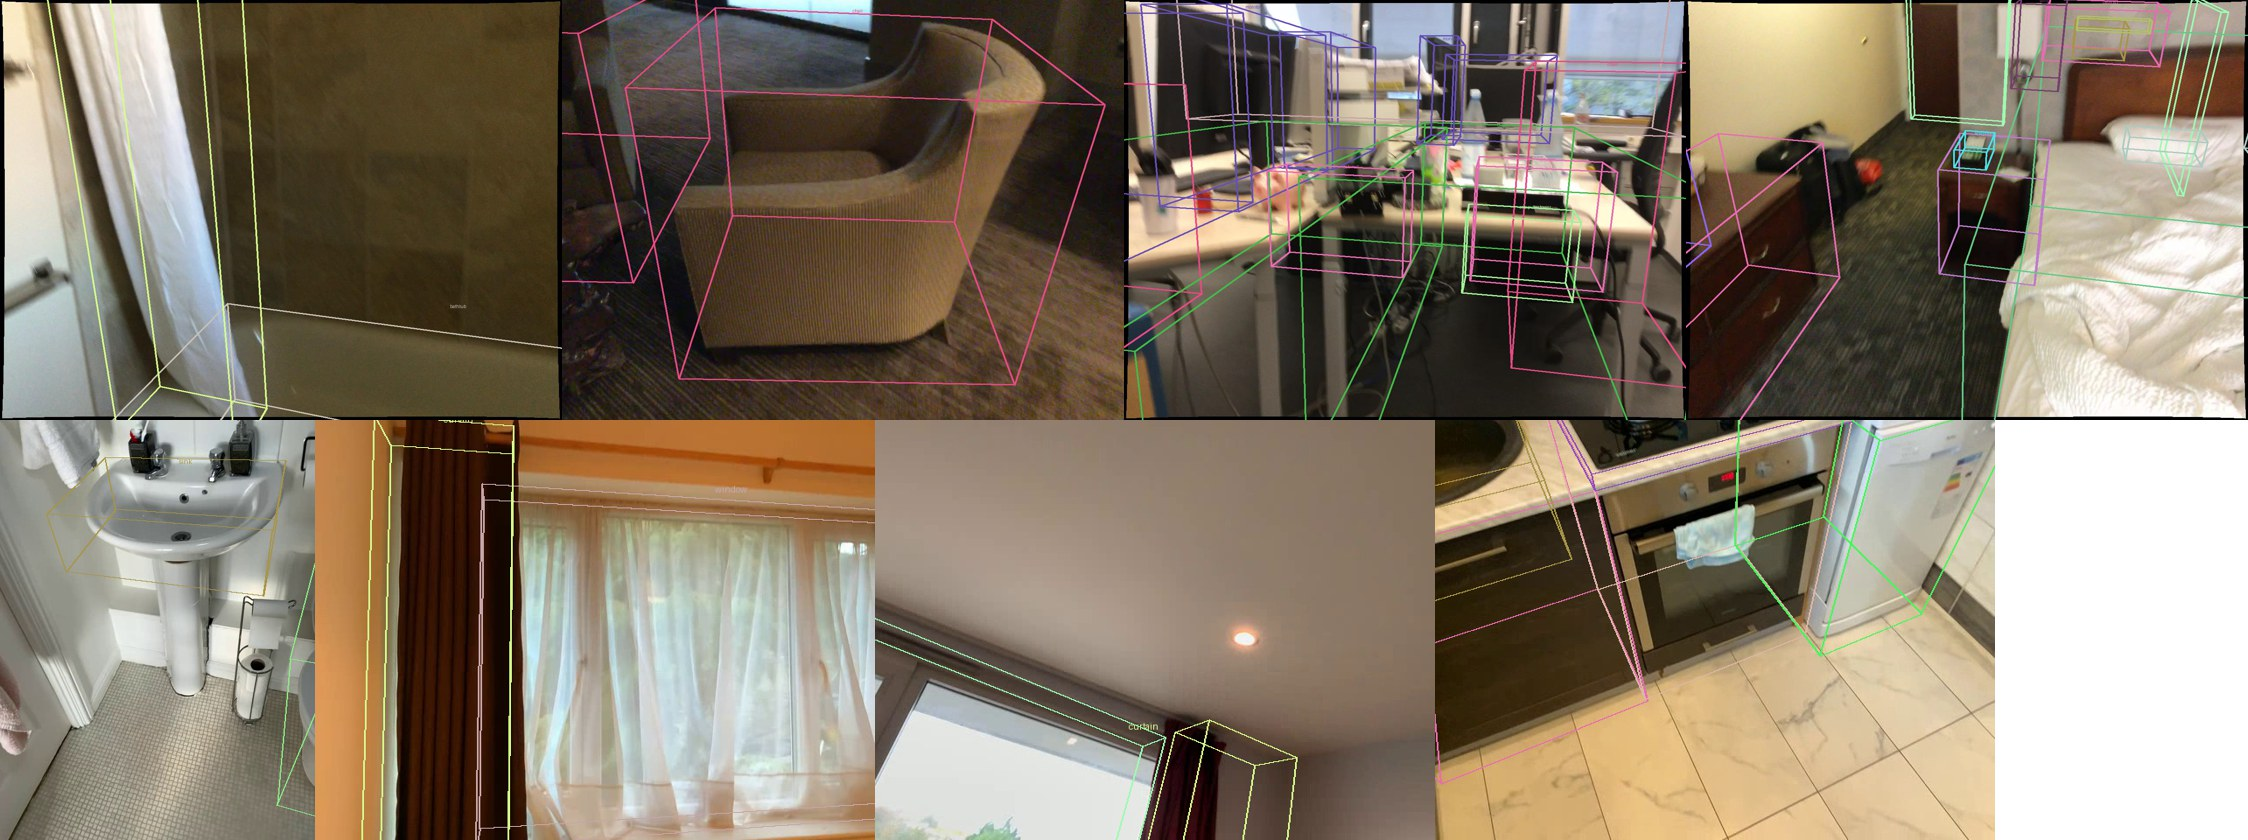
\includegraphics[width=\linewidth]{vggt-det-training-data-overlay.jpg}
\caption{Ground-truth boxes projected into the images with the stored alignment matrix, pose and intrinsics.
Top: ScanNet. Bottom: ARKitScenes after the correction.}
\label{fig:vggtdet-overlay}
\end{figure}

\subsection{Corrections}
\label{sec:vggtdet-data-fix}

\paragraph{Origin.}
For each ARKitScenes scene the alignment matrix gets an extra translation that moves the mean $x$, $y$ of the
points to 0 and their 2nd $z$ percentile (the floor) to 0; the boxes move with it. The median shift is 0.85,
1.87 and 1.23\,m in $x$, $y$ and $z$. The rotation is untouched. Box centres expressed in the scene's world
frame, and hence in every camera's frame, change by less than $10^{-14}$\,m, and sizes do not change.

\paragraph{Focal length.}
Portrait scenes whose focal length is below 0.72 of the long image side (the camera's true value is 0.82 to
0.85) get it multiplied by height over width. This applies to 1,031 of 2,267 training scenes and 265 of 562
validation scenes. Applying either correction a second time changes nothing.

\paragraph{Scope.}
The corrections are applied to the ARKitScenes training and validation files of the 63-class detector and are
built into the two converters that write such files. The files used for inference on Reason-190K and
VSI-Bench keep the first-camera origin on purpose, because the downstream code expects the detections in that
frame. Their portrait focal lengths are still too small; the detector does not read them, but the converter
that writes them (\texttt{build\_arkit\_inputs.py}) should scale by the long image side.
